\section{Application architecture}\label{sec:architecture}

On the basis of objectives it is possible to design architecture of the application

The architecture of the application is influenced by two fundamental factors:

\begin {enumerate}
\item the Application has to be cross-platform for a mobile operating system.
\item Application will be used with different CRM systems.
\end {enumerate}

The first factor divides architecture of the application into two parts. The first part is platform-independent and can be realized by means of a cross platform framework. The second part is the code written with aiming at a certain operating system. The second part has to be as little as possible to exclude realization of the same methods repeatedly.

\subsection{Platform-dependent part}

In a platform-dependent part of the application two functions have to be realized.

The first function is an application launch in the background. The background mode is necessary so the application could monitor the events related with calls even when the application is closed. The incoming and outgoing calls can be made in the way, habitual for the user, – from the notebook. These calls also have to be processed by the application.

The second function is related to a call event. The application has to be able to react to an event of the ending of a call and to obtain information about it. After obtaining the necessary information, the process of checking the base of clients for the phone number has to be initiated.

\subsection{Cross-platform part}

First of all, the graphic interface belongs here. The chosen cross platform cursor of Xamarin allows creating the graphic interface common for all platforms. During the compilation of the application under a certain operating system also the graphic interface will be compiled.

The main logic of the application belongs to a cross-platform part. Further some tasks which are carried out in this part are presented.

\begin {itemize}
\item Data read-out from the fields filled with the user.
\item Call of authorization function.
\item Saving correct data of authorization and, further, verification of that data.
\item Request of the list of clients, its display in the graphic interface.
\item Comparison of phone number, from which a call was made, with numbers from base of contacts.
\end {itemize}

The architecture of the application is presented on picture \ref {fig:appArchitecture}.

\begin{figure}[tbh]
\centering
\caption{Applications architecture}
\label{fig:appArchitecture}
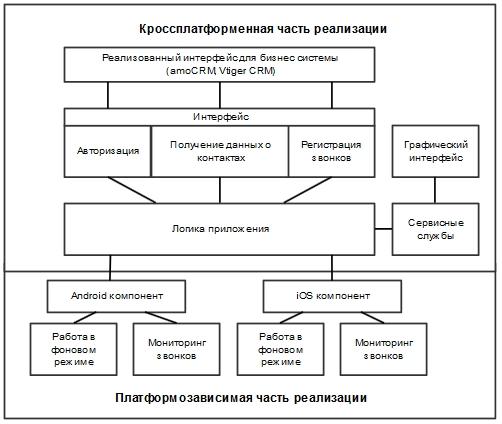
\includegraphics[width=\linewidth]{appArchitecture}
\end{figure}